\section{Tournois}

Cette section explique comment s'inscrire à un tournoi, ou annuler une inscription à un tournoi.

\subsection{S'inscrire à un tournoi}

Pour vous inscrire à un tournoi, vous devez cliquer aller sur la page "Tournois", disponible uniquement pour les utilisateurs connecté. Ensuite, vous devez cliquer sur le bouton "S'inscrire à un tournoi", en bas de la page.

\begin{figure}[H]
\centering
\includegraphics[scale=0.15]{user_images/basic_user/GererTournois/InscriptionComplete/001.jpg}
\caption{Inscription à un tournoi, étape 1}
\end{figure}

Sur cette page d'inscription au tournoi, vous avez un module de recherche d'utilisateurs à gauche, et un formulaire d'inscription à droite. \newline

Pour commencer l'inscription, vous devez d'abord choisir un partenaire avec qui jouer. Pour choisir un partenaire, vous devez sélectionner un utilisateur à gauche parmi la liste des utilisateurs disponibles. Vous pouvez affiner la liste en remplisant le champs de recherche, ou en accédant aux pages de la recherche suivante.\newline

\begin{figure}[H]
\centering
\includegraphics[scale=0.15]{user_images/basic_user/GererTournois/InscriptionComplete/002.jpg}
\caption{Inscription à un tournoi, étape 2}
\end{figure}

Dès que vous avez sélectionné un utilisateur, le formulaire détecte automatiquement le tournoi associé à l'inscription, comme indiqué en haut à droite de la page. Ensuite, vous pouvez choisir les extras que vous voulez, et entrer un commentaire si vous avez des remarques ou des souhaits particuliers concernant le déroulement du tournoi.\newline

Veuillez remarquer que vous ne pouvez pas sélectionner les extras du 2ème joueur. En effet, c'est à lui de les choisir au moment de valider la demande d'inscription (étape 6).

\begin{figure}[H]
\centering
\includegraphics[scale=0.15]{user_images/basic_user/GererTournois/InscriptionComplete/003.jpg}
\caption{Inscription à un tournoi, étape 3}
\end{figure}

Pour confirmer l'inscription au tournoi, lorsque vous avez choisi un partenaire, vous pourrez cliquer sur le bouton "Inscription" en bas de la page.

\begin{figure}[H]
\centering
\includegraphics[scale=0.15]{user_images/basic_user/GererTournois/InscriptionComplete/004.jpg}
\caption{Inscription à un tournoi, étape 4}
\end{figure}

L'inscription au tournoi est en cours. Pour continuer, le partenaire doit valider votre demande d'inscription.

\begin{figure}[H]
\centering
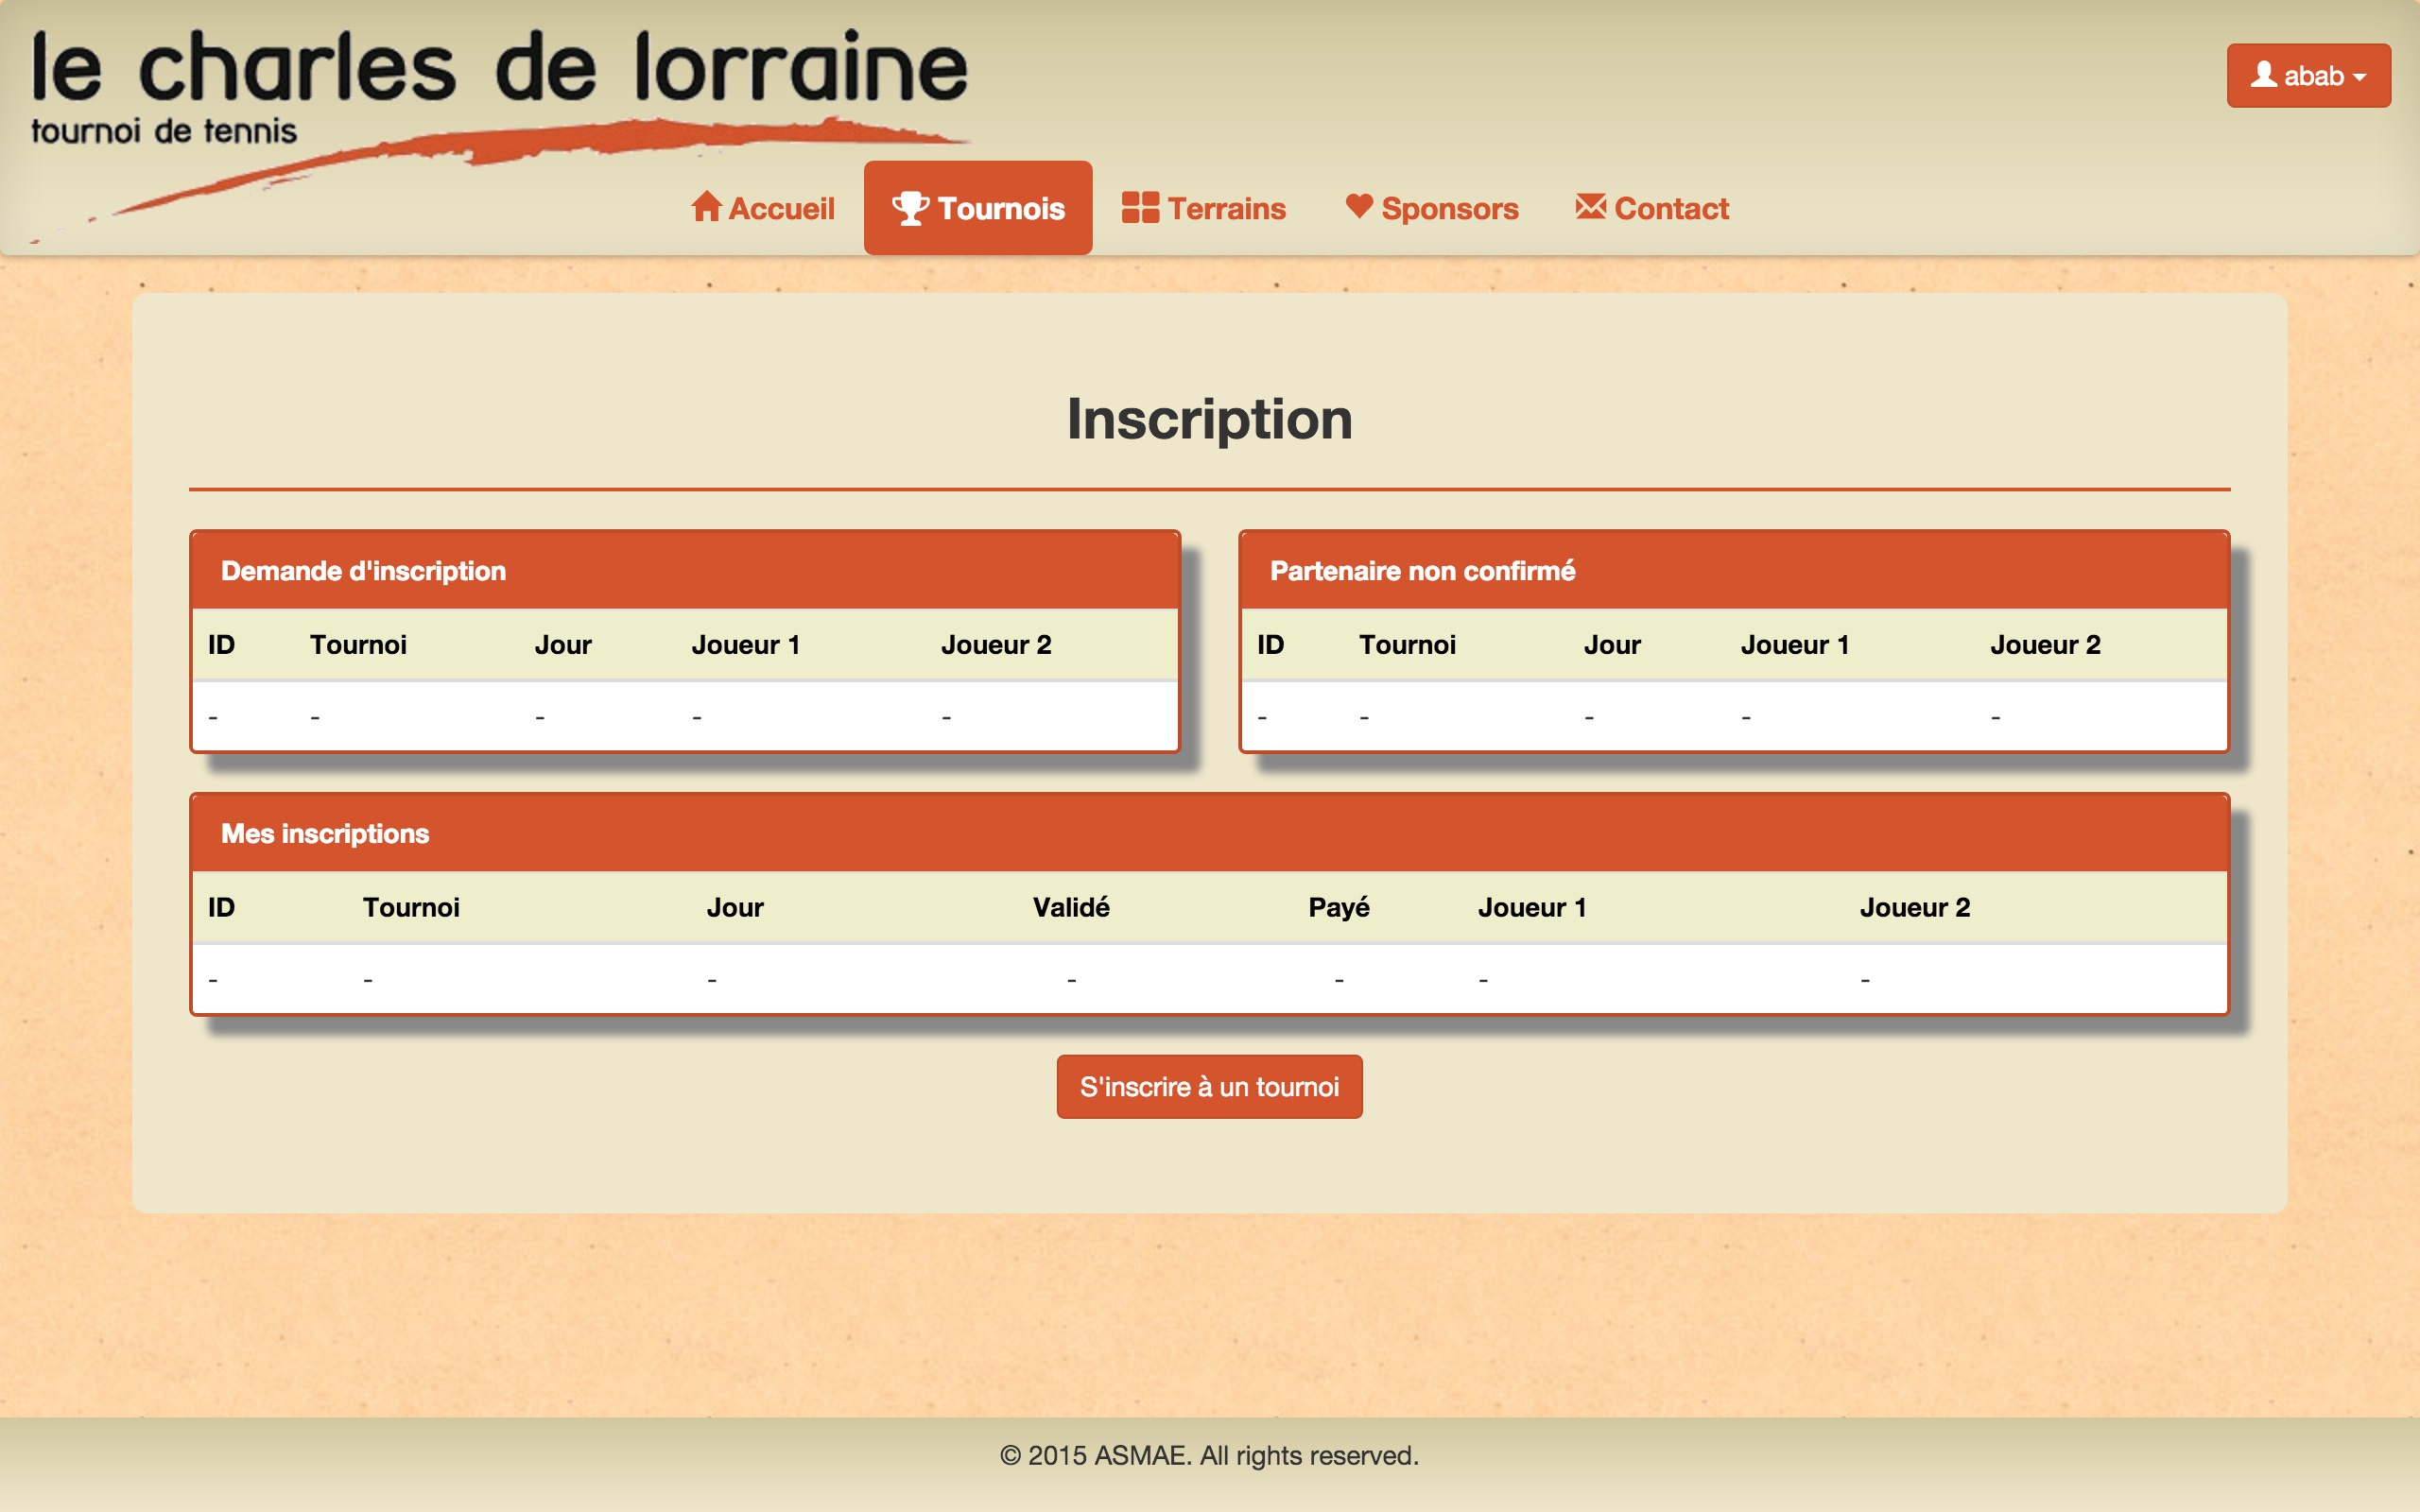
\includegraphics[scale=0.15]{user_images/basic_user/GererTournois/InscriptionComplete/005.jpg}
\caption{Inscription à un tournoi, étape 5}
\end{figure}

Du côté du partenaire, il peut consulter ses demande d'inscription à un tournoi. Celui-ci peut accepter ou refuser la demande d'inscription. \newline

S'il accepte la demande d'inscription, il peut sélectionner les extras et ajouter des remarques ou souhaits avant la confirmation d'inscription de la paire de joueurs.

\begin{figure}[H]
\centering
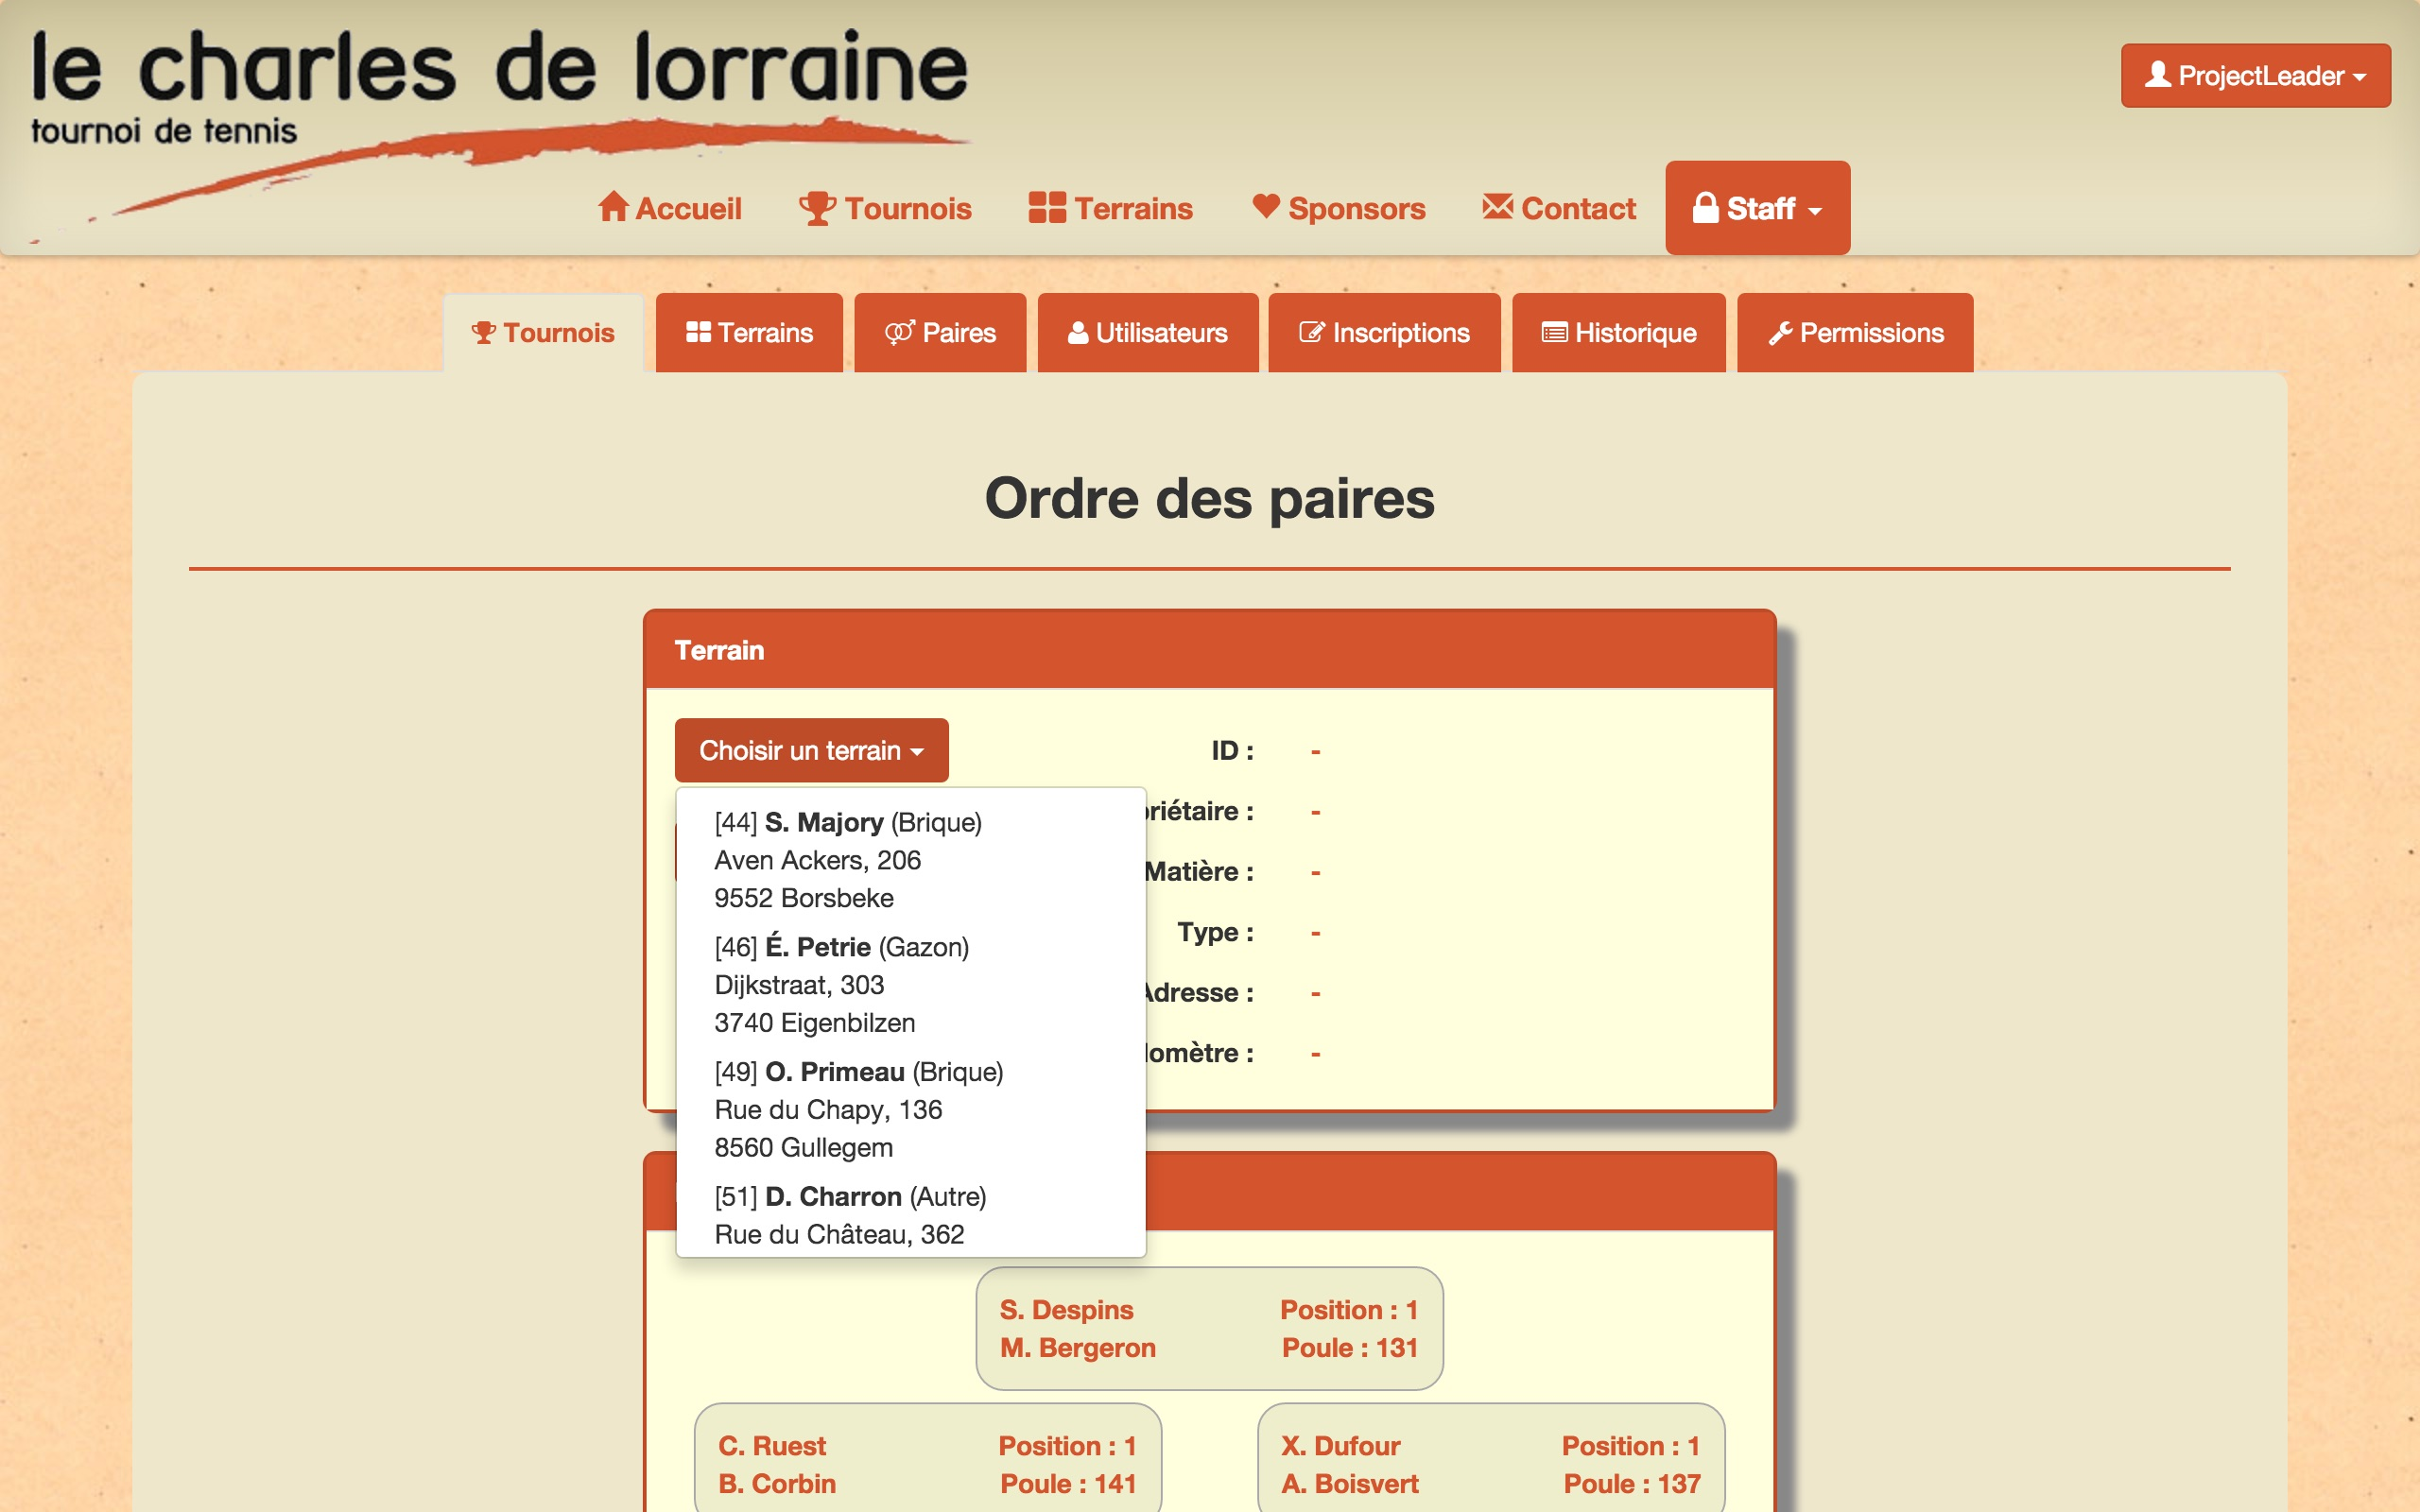
\includegraphics[scale=0.15]{user_images/basic_user/GererTournois/InscriptionComplete/006.jpg}
\caption{Inscription à un tournoi, étape 6}
\end{figure}

Après avoir sélectionner les extras et/ou ajouter un commentaire, cliquer sur "Valider" pour accepter la demande d'inscription au tournoi en paire.

\begin{figure}[H]
\centering
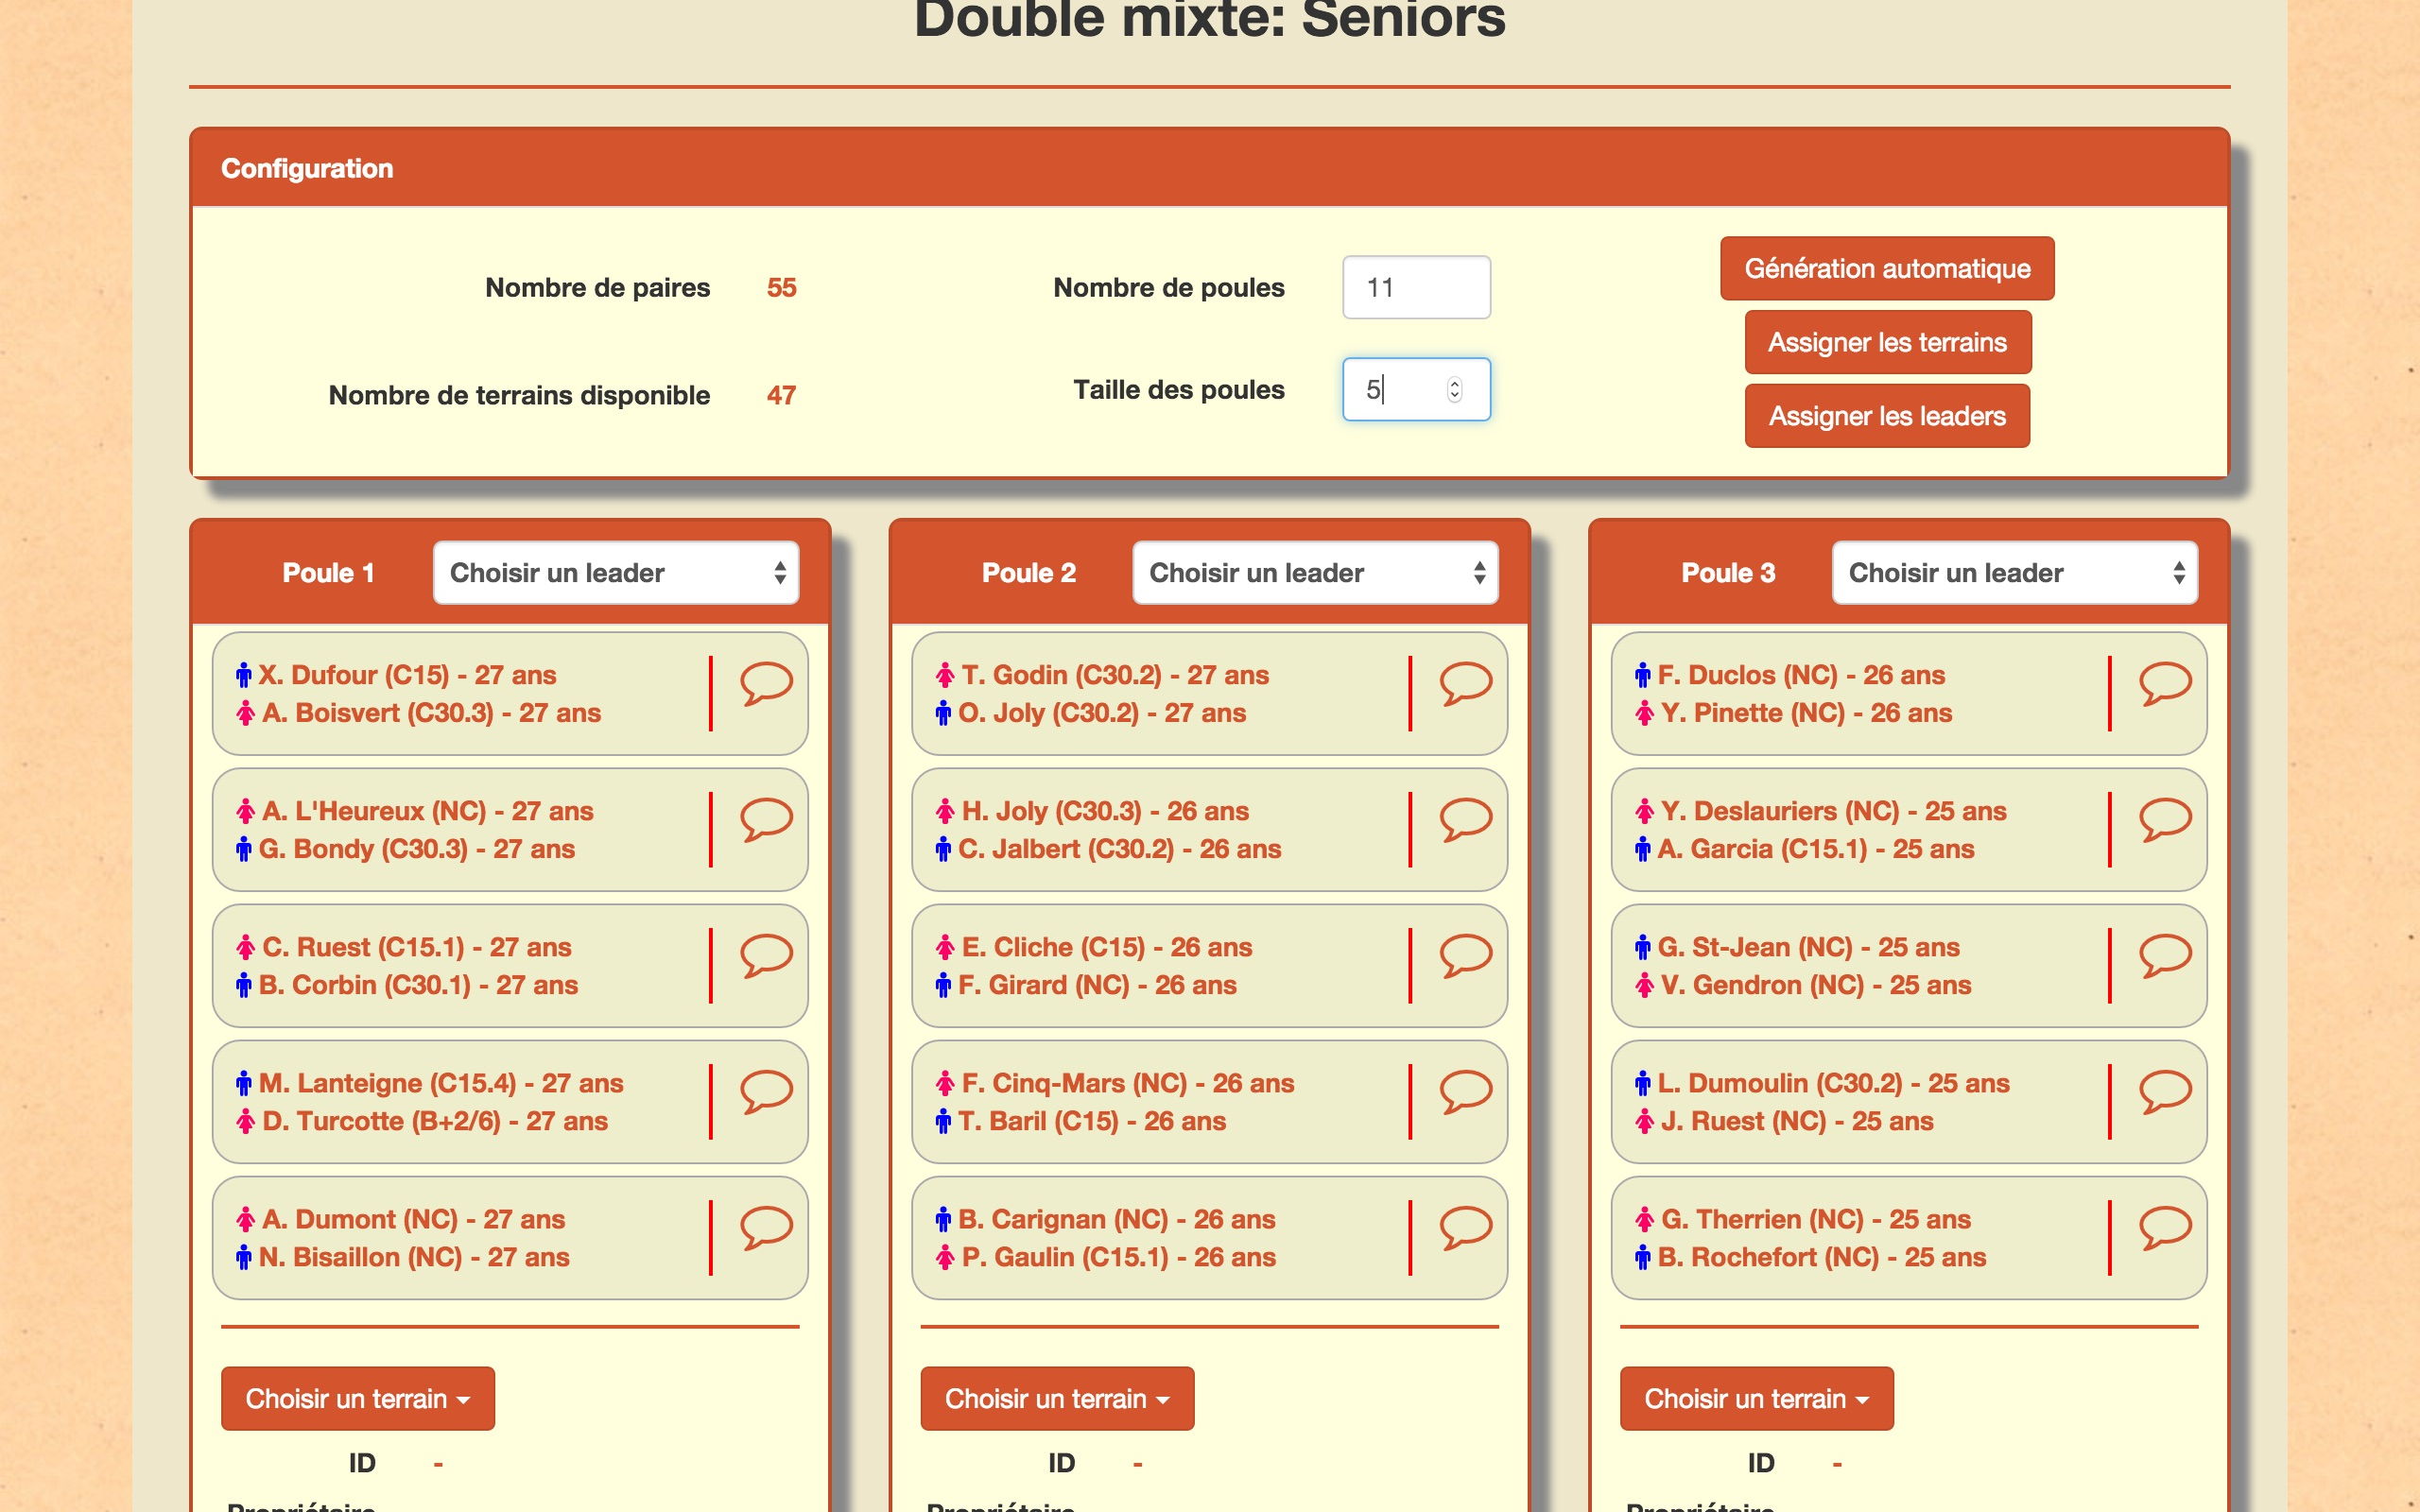
\includegraphics[scale=0.15]{user_images/basic_user/GererTournois/InscriptionComplete/007.jpg}
\caption{Inscription à un tournoi, étape 7}
\end{figure}

L'inscription de la paire est pratiquemment terminée. Il suffit plus qu'un membre du staff valide la paire.

\begin{figure}[H]
\centering
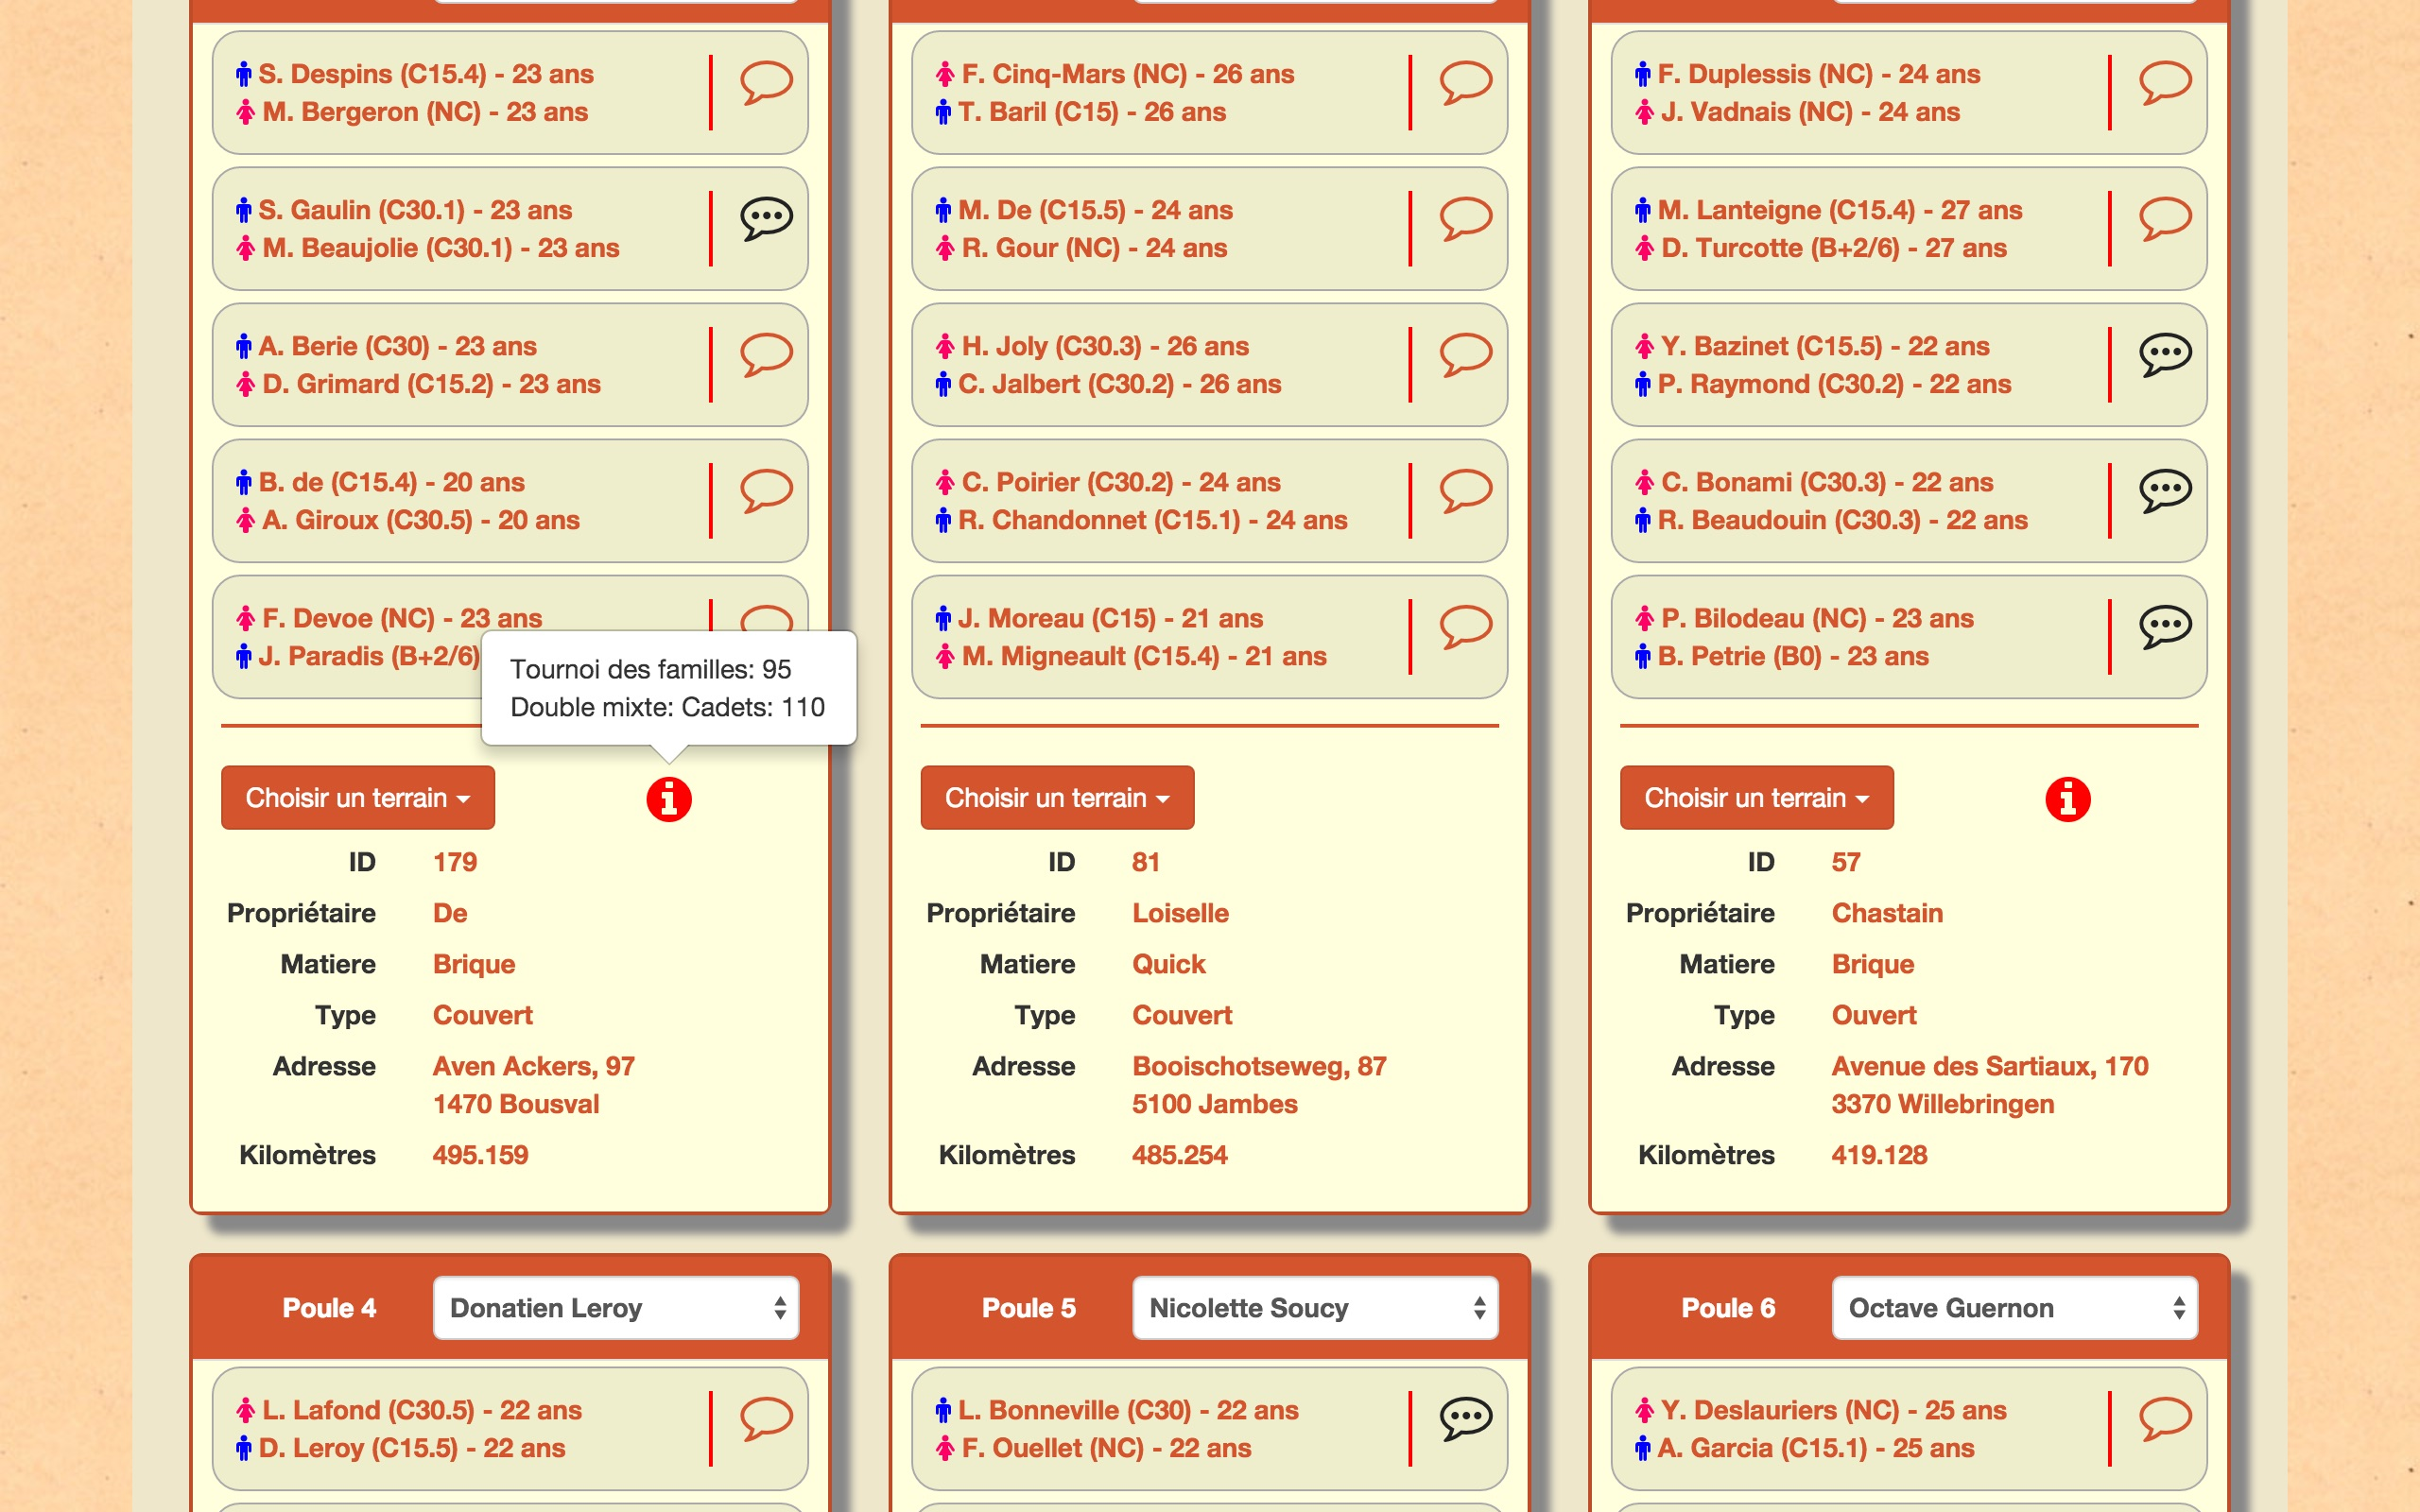
\includegraphics[scale=0.15]{user_images/basic_user/GererTournois/InscriptionComplete/008.jpg}
\caption{Inscription à un tournoi, étape 8}
\end{figure}

Dès qu'un membre du staff a validé la paire, celle-ci participera au tournoi inscrit.

\begin{figure}[H]
\centering
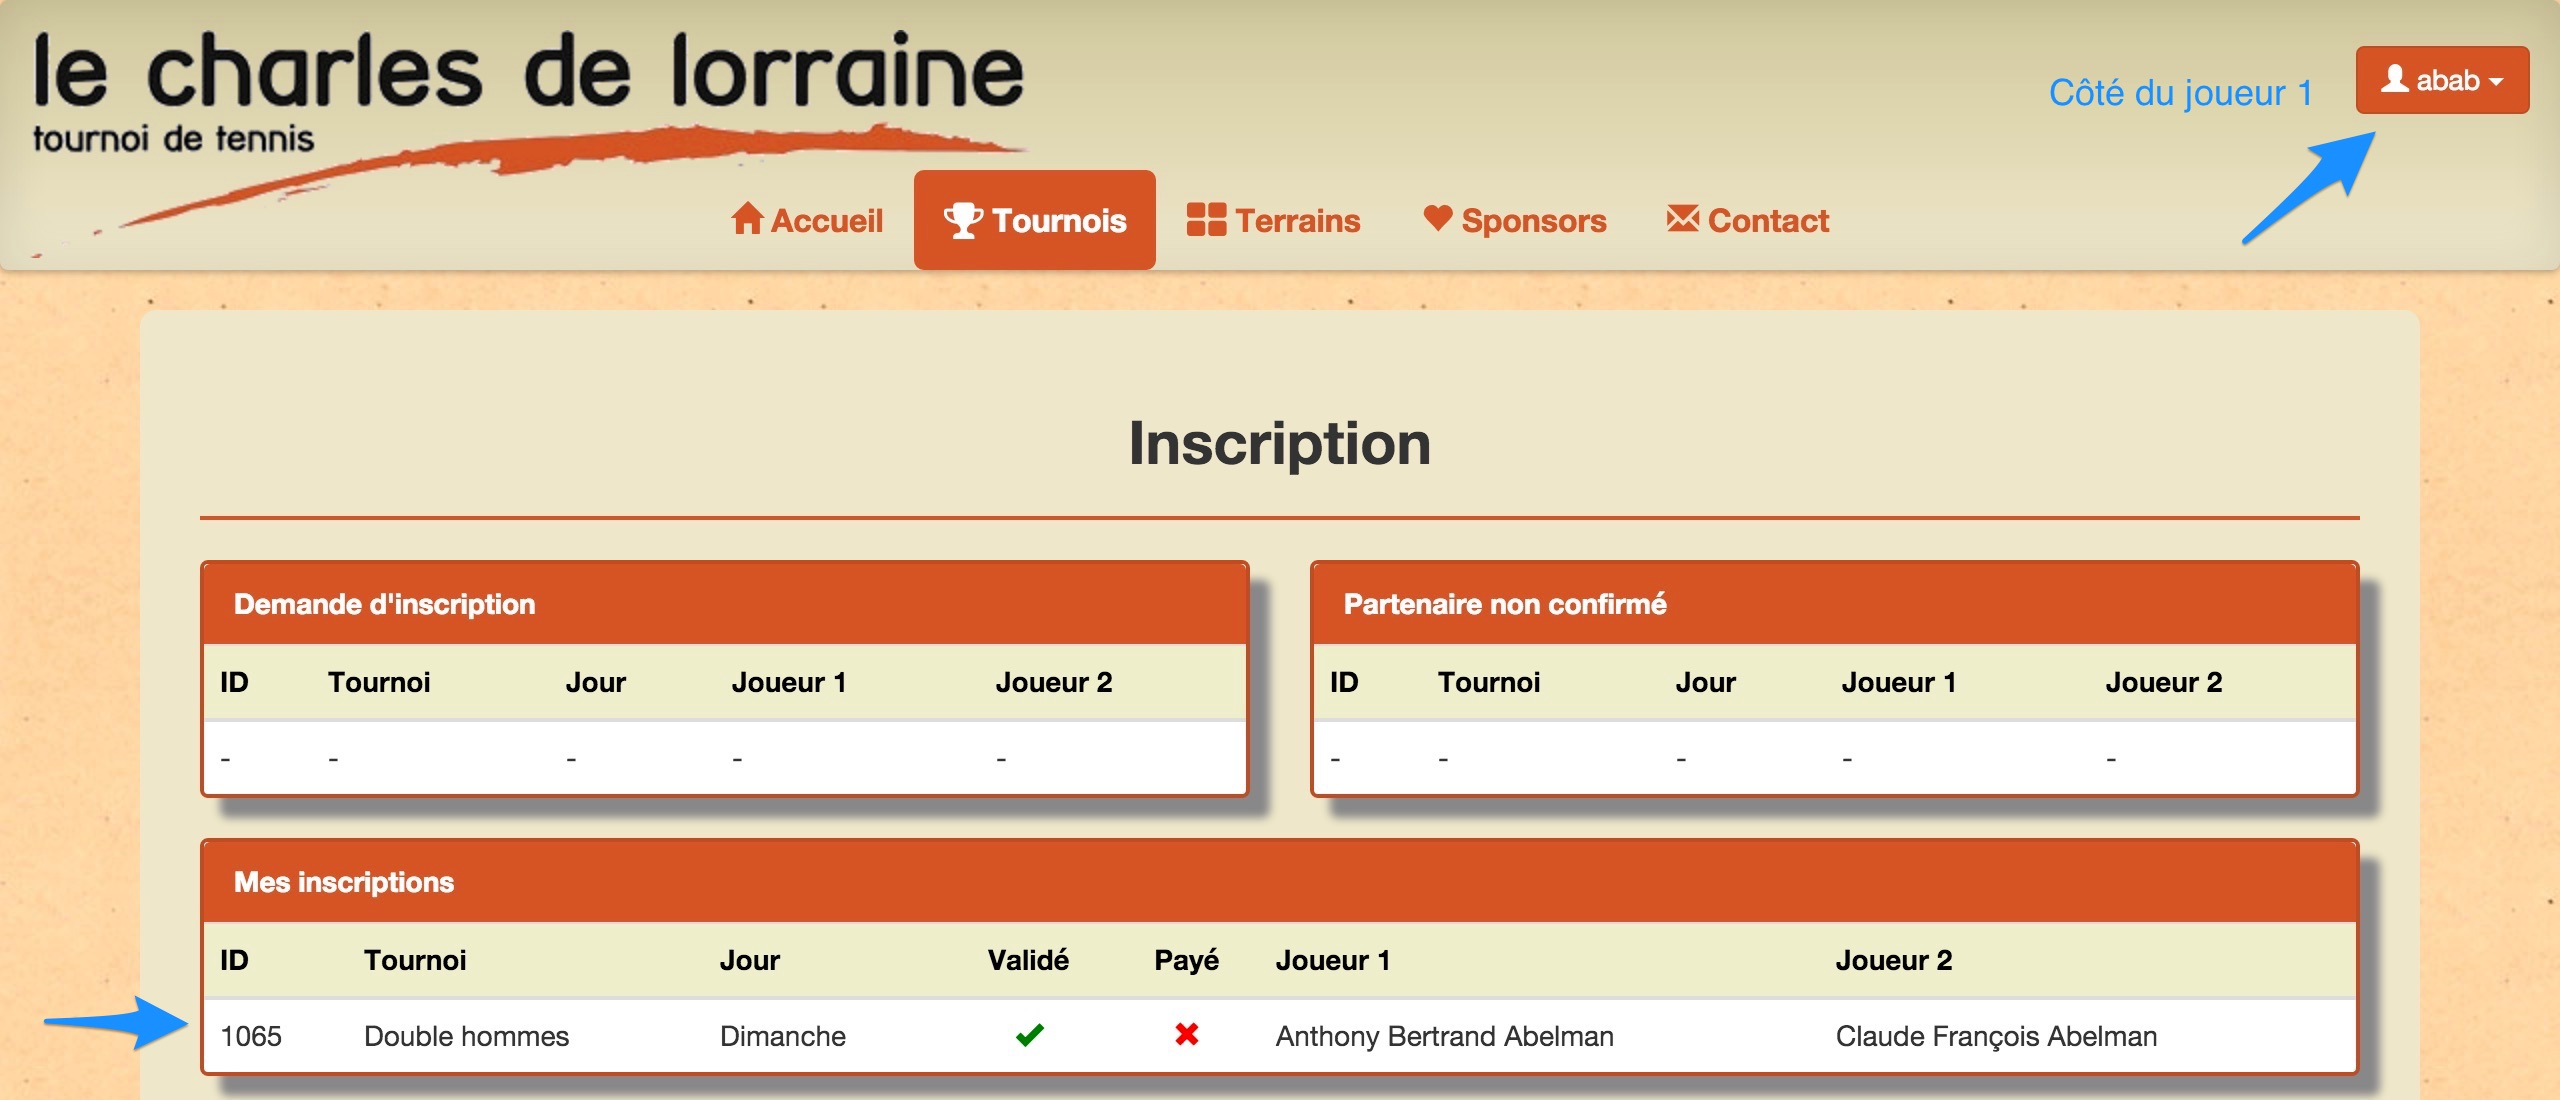
\includegraphics[scale=0.15]{user_images/basic_user/GererTournois/InscriptionComplete/009.jpg}
\caption{Inscription à un tournoi, étape 9}
\end{figure}

\subsection{Annuler inscription à un tournoi}

Il est possible d'annuler l'inscription, par un utilisateur standard, à un tournoi lorsque le deuxième joueur n'a pas accepté l'inscription en paire.\newline

Pour le 1er joueur, il suffit de consulter ses inscriptions en cours de confirmation de la part du 2ème joueur, en cliquant sur la paire temporairement créée dans la liste en haut à droite de la page.

\begin{figure}[H]
\centering
\includegraphics[scale=0.15]{user_images/basic_user/GererTournois/AnnulerInscription/AnnulerDemandeJoueur1/001.jpg}
\caption{Annulation inscription tournoi par joueur 1, étape 1}
\end{figure}

Sur la page de la demande de paire, il est possible d'annuler la demande d'inscription de la paire en cliquant sur le bouton "Supprimer".

\begin{figure}[H]
\centering
\includegraphics[scale=0.15]{user_images/basic_user/GererTournois/AnnulerInscription/AnnulerDemandeJoueur1/002.jpg}
\caption{Annulation inscription tournoi par joueur 1, étape 2}
\end{figure}

Cette action est irréversible. Une boîte de dialogue demande à l'utilisateur de confirmer son choix de suppression de la paire en cours d'inscription.

\begin{figure}[H]
\centering
\includegraphics[scale=0.15]{user_images/basic_user/GererTournois/AnnulerInscription/AnnulerDemandeJoueur1/003.jpg}
\caption{Annulation inscription tournoi par joueur 1, étape 3}
\end{figure}

Si l'utilisateur confirme son souhait d'annuler son inscription, il sera bien désinscrit du tournoi.

\begin{figure}[H]
\centering
\includegraphics[scale=0.15]{user_images/basic_user/GererTournois/AnnulerInscription/AnnulerDemandeJoueur1/004.jpg}
\caption{Annulation inscription tournoi par joueur 1, étape 4}
\end{figure}

Le joueur 2 peut aussi annuler l'inscription à un tournoi en refusant une demande d'inscription. Sur sa page de tournoi, il peut consulter à la demande de confirmation de la paire en cliquant sur la demande souhaitée, en haut à gauche de la page.

\begin{figure}[H]
\centering
\includegraphics[scale=0.15]{user_images/basic_user/GererTournois/AnnulerInscription/AnnulerDemandeJoueur2/001.jpg}
\caption{Annulation inscription tournoi par joueur 2, étape 1}
\end{figure}

Ensuite, au lieu de choisir ses extras, écrire un commentaire, et accepter la demande, celui-ci peut cliquer sur le bouton "Refuser" pour refuser la demande d'inscription au tournoi.

\begin{figure}[H]
\centering
\includegraphics[scale=0.15]{user_images/basic_user/GererTournois/AnnulerInscription/AnnulerDemandeJoueur2/002.jpg}
\caption{Annulation inscription tournoi par joueur 2, étape 2}
\end{figure}

Comme cette action est irréversible, il est demandé à l'utilisateur de confirmer son choix de refuser la demande d'inscription au tournoi.

\begin{figure}[H]
\centering
\includegraphics[scale=0.15]{user_images/basic_user/GererTournois/AnnulerInscription/AnnulerDemandeJoueur2/003.jpg}
\caption{Annulation inscription tournoi par joueur 2, étape 3}
\end{figure}

L'inscription au tournoi sera bien annulé.

\begin{figure}[H]
\centering
\includegraphics[scale=0.15]{user_images/basic_user/GererTournois/AnnulerInscription/AnnulerDemandeJoueur2/004.jpg}
\caption{Annulation inscription tournoi par joueur 2, étape 4}
\end{figure}

\subsection{Payer son inscription}

Pour effectuer le paiement de la paire à l'inscription à un tournoi, l'un des deux joueurs de la paire doit consulter les informations de la paire, en cliquant sur sur l'inscription dans la liste des inscriptions, sur la page "Tournois".

\begin{figure}[H]
\centering
\includegraphics[scale=0.15]{user_images/basic_user/GererTournois/PaiementInscription/001.jpg}
\caption{Paiement inscription au tournoi, étape 1}
\end{figure}

Ensuite, il doit cliquer sur le bouton "Payer", en bas de la page.

\begin{figure}[H]
\centering
\includegraphics[scale=0.15]{user_images/basic_user/GererTournois/PaiementInscription/002.jpg}
\caption{Paiement inscription au tournoi, étape 2}
\end{figure}

Sur cette page, l'utilisateur peut consulter le coût total de l'inscription de la paire, ainsi que choisir le mode de paiement vous payer l'inscription. Plusieurs modes de paiement sont disponibles, comme Visa, Paypal, ou Mastercard.

\begin{figure}[H]
\centering
\includegraphics[scale=0.15]{user_images/basic_user/GererTournois/PaiementInscription/003.jpg}
\caption{Paiement inscription au tournoi, étape 3}
\end{figure}

Lorsque la paire aura payé son inscription, et que le staff aura bien reçu l'information du paiement, un membre du staff indiquera que la paire a bien payée son inscription.

\begin{figure}[H]
\centering
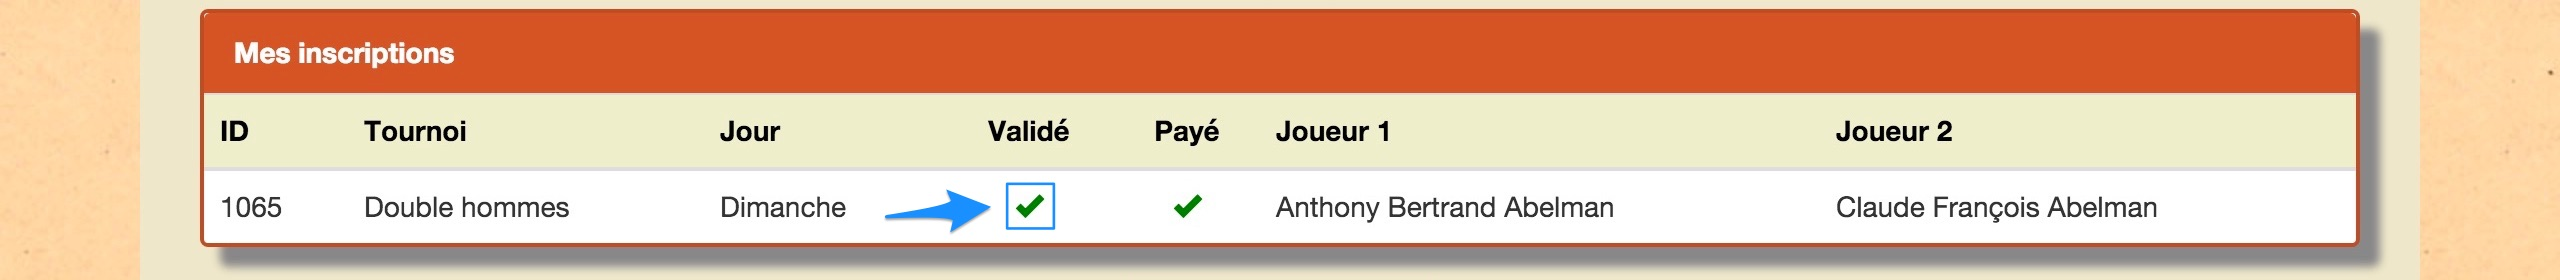
\includegraphics[scale=0.15]{user_images/basic_user/GererTournois/PaiementInscription/au_final.jpg}
\caption{Paiement inscription au tournoi, étape finale}
\end{figure}